\begin{comment}
\documentclass[10pt]{article}
\usepackage{fullpage, graphicx, url}
\setlength{\parskip}{1ex}
\setlength{\parindent}{0ex}
\title{GEN10}
\begin{document}


\begin{tabular}{ccc}
The Alternative Csound Reference Manual & & \\
Previous & &Next

\end{tabular}

%\hline 
\end{comment}
\section{GEN10}
GEN10�--� Generate composite waveforms made up of weighted sums of simple sinusoids. \subsection*{Description}


  These subroutines generate composite waveforms made up of weighted sums of simple sinusoids. The specification of each contributing partial requires 1 pfield using \emph{GEN10}
. 
\subsection*{Syntax}


 \textbf{f}
 \# time size 10 str1 str2 str3 str4 ...
\subsection*{Initialization}


 \emph{size}
 -- number of points in the table. Must be a power of 2 or power-of-2 plus 1 (see \emph{f statement}
). 


 \emph{str1, str2, str3, etc.}
 -- relative strengths of the fixed harmonic partial numbers 1,2,3, etc., beginning in p5. Partials not required should be given a strength of zero. 


 


\begin{tabular}{cc}
\textbf{Note}
 \\
� &

 


 
\begin{itemize}
\item 

  These subroutines generate stored functions as sums of sinusoids of different frequencies. The two major restrictions on \emph{GEN10}
 that the partials be harmonic and in phase do not apply to \emph{GEN09}
 or \emph{GEN19}
. 


  In each case the composite wave, once drawn, is then rescaled to unity if p4 was positive. A negative p4 will cause rescaling to be skipped. 


\end{itemize}


\end{tabular}

\subsection*{Examples}


  Here is a simple example of the GEN10 routine. It uses the files \emph{gen10.orc}
 and \emph{gen10.sco}
. It will generate a simple sine wave. Here is its diagram: 


 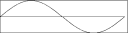
\includegraphics[scale=1]{gen10} 


 Diagram of the waveform generated by GEN10.


 \textbf{Example 1. A simple example of the GEN10 routine.}

\begin{lstlisting}
/* gen10.orc */
; Initialize the global variables.
sr = 44100
kr = 4410
ksmps = 10
nchnls = 1

; Instrument #1.
instr 1
  kamp = 30000
  kcps = 440
  ifn = 1

  ; Play the sine wave stored in Table #1.
  a1 oscil kamp, kcps, ifn
  out a1
endin
/* gen10.orc */
        
\end{lstlisting}
\begin{lstlisting}
/* gen10.sco */
; Table #1: a simple sine wave (using GEN10).
f 1 0 16384 10 1

; Play Instrument #1 for 2 seconds.
i 1 0 2
e
/* gen10.sco */
        
\end{lstlisting}
\subsection*{See Also}


 \emph{GEN09}
, \emph{GEN11}
, and \emph{GEN19}
. 
\subsection*{Credits}


 Example written by Kevin Conder
%\hline 


\begin{comment}
\begin{tabular}{lcr}
Previous &Home &Next \\
GEN09 &Up &GEN11

\end{tabular}


\end{document}
\end{comment}
